\subsection{Introduction}

Data compression or source coding is the process of encoding information using fewer bits. There are two main classes of data compression; lossless and lossy. Lossless data compression does not lose information in the process of encoding. Rather, it eliminates statistical redundancy or `wasted space' in the information source. On the other hand, lossy data compression partially discards information such that the original data cannot be fully reconstructed. For this reason, lossy compression is also known as irreversible compression.

%Many data compression techniques have been developed since the inception of information theory in the 1920s. Lossless compression techniques can be broadly categorised into three encoding methods; entropy, dictionary and other types.

%\def\lossless{(0,0) circle (4cm)}
%\def\lossy{(0,4) circle (4cm)}
%\def\entropy{(180:2cm) circle (2cm)}
%\def\dict{(0:2cm) circle (2cm)}
%
%% Now we can draw the sets:
%\begin{tikzpicture}
%\draw \data node[below] {Lossless};
%\draw \entropy node [above] {Entropy};
%\draw \dict node [below] {Dictionary};
%\end{tikzpicture}

% TODO compression classes venn diagram

Data compression relies on the framework of information theory established fundamentally by Claude E. Shannon in ``A Mathematical Theory of Communication'' \cite{shannon}. Information theory studies the transmission of digital information through communication systems. The communication system Shannon theorises is composed of five parts: the information source, transmitter, channel, receiver and destination. See Figure \ref{fig:shannon-comm-system}. Depending on the information transmitted through the system, it is classified into three main categories; discrete, continuous and mixed.

\begin{figure}
\centering
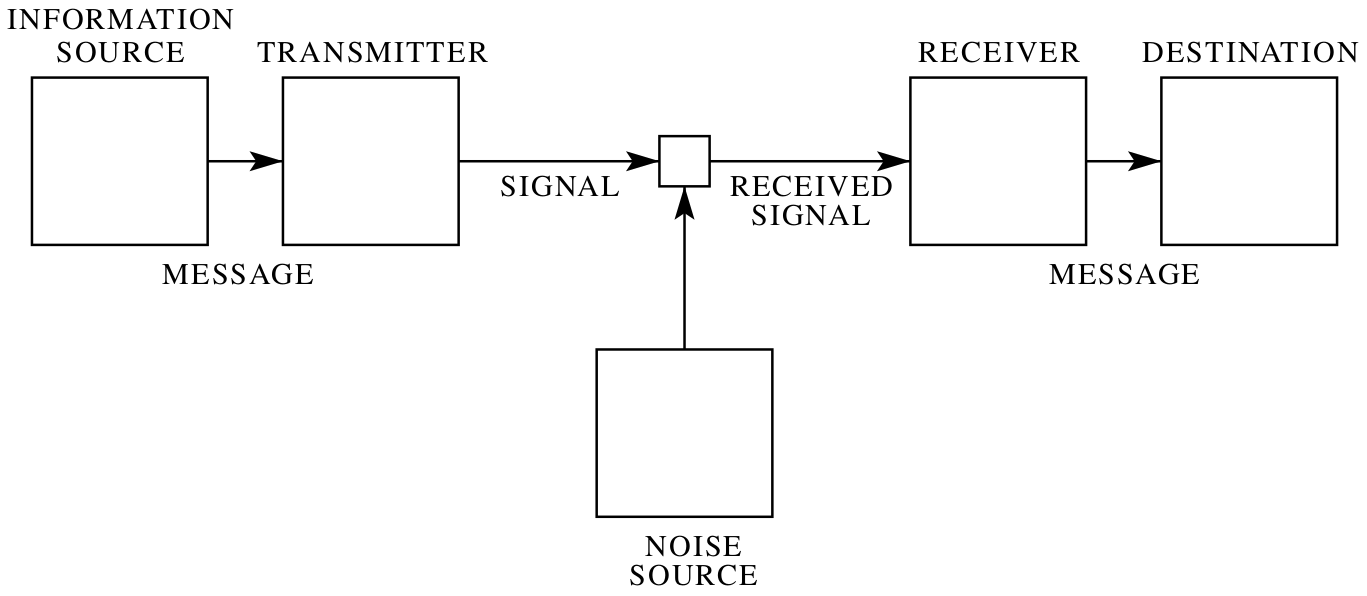
\includegraphics[scale=0.25]{plots/shannon-comm-system.png}
\caption[Shannon's general communication system.]{\label{fig:shannon-comm-system}Shannon's general communication system consists of
an \textit{information source} which produces a message,
a \textit{transmitter} which manipulates the message to produce a signal suitable for transmission over the channel,
a \textit{channel} which serves as the medium for signal transmission from the transmitter to the receiver,
a \textit{receiver} which reconstructs the message from the signal and
a \textit{destination} which is the message's intended point of delivery\protect\footnotemark[2].}
\end{figure}

\footnotetext[1]{Figure \ref{fig:shannon-comm-system} was taken from Fig. 1 in \cite{shannon}.}

In the discrete case, the information source can be represented by a stochastic process \[\{X_t: t\in\mathbb{N}^+\}\] with a discrete state space $S$. Governed by this mathematical model, the information source produces a sequence of symbols from its alphabet which is received by the transmitter. If the probability of the transmitter observing the next symbol depends only on the current symbol and is conditionally independent of previous symbols, the process satisfies the Markov property. In this case, the information source can be represented by a Markov chain with a finite state space $S_1,S_2,\dots,S_n$ and a set of transition probabilities $p_i(j)$ defined as the probability that the system will transition from state $S_i$ to $S_j$.

The entropy rate, $H$, of an information source is a measure of how much information it `produces' per symbol on average. Or rather, how uncertain the transmitter is of the next symbol on average. It is strictly positive unless we are certain of the outcome in which case it is 0. For a discrete random variable $X$ where each symbol $s_1,s_2,\dots,s_n$ is independent of the next; the entropy is given by \[H(X)=-\sum_{i=1}^np_i\log_2p_i\] where $p_i$ is the probability of observing the $i$-th symbol \cite{shannon}. The units here are in bits. For an information source represented as a stochastic process, the entropy rate is given by \[H(X)=\lim_{n\to\infty}\frac{1}{n}H(X_1,X_2,\dots,X_n)\] when the limit exists, where $H(X_1,X_2,\dots,X_n)$ is the joint entropy of the first $n$ members of the process \cite{info-book}. The limit is known to exist for a stationary process where the joint probability distribution is invariant to shifts in time. For example, for a stationary Markov chain the entropy rate simplifies to \[H(X)=-\sum_{i,j}\mu_ip_i(j)\log_2p_i(j)\] where $\mu$ is the stationary distribution of the chain.

% TODO example of calculated entropy and markov chain

The Hartley function $H_0$ or absolute rate $R$ of an alphabet $S$ is the maximum possible entropy rate that can be achieved using it. It is defined as the logarithm of the alphabet's cardinality
\[ H_0(S)=R=log_2|S|.\]

% TODO redundancy and maximum compression

A binary source code, $C$, of a random variable $X$ is a mapping from its possible outcomes $\Omega$ to a set of finite length strings of symbols from $\{0,1\}$ known as codewords. A code is described as a prefix code or instantaneous code when no codeword is a prefix of another. In such a case, any encoded string can be conveniently decoded without reference to future codewords. For uniquely decodable codes, the expected length of a codeword cannot be smaller than the entropy of $X$. That is, \[\sum_i p_il_i\ge H(X)\] where $l_i=|C(s_i)|$ is the length of the $i$-th symbol's codeword. With equality possible if and only if the probability distribution is dyadic. That is, when $\forall i\;\exists n\in\mathbb{N}_0$ such that $p_i=2^{-n}$. Similarly, the entropy rate also defines a lower limit on the expected number of bits per symbol for a source encoding of an information source represented as a stochastic process.%This is closely related to Shannon's source coding theorem.

%There are several enveloping classes of codes as displayed in Figure~\ref{fig:codes}.
% TODO codes figure

%According to Shannon's source coding theorem, the code rate (average number of bits per symbol) of a lossless source encoding.
%That is, given $M:S\to \{0,1\}$, a mapping from symbols to bits \[H(X)\le\lim_{n\to\infty}\frac{1}{n}\sum_{i=1}^nM(X_i)\]
